\chapter{Lifetime-Limited Memory}
\label{llmchap}
In this section, we will describe the structure of the Lifetime Limited Memory model developed through the course of the project. We consider a network with $n_c$ classes, $n_h$ hidden units, and $n_t$ log-linear spaced timescales. The LLM takes as input a sequence of event labels, and outputs for the a specified task as described in \ref{tasks}. Let $X_{train}$ be the training set with $N$ data points. Let $x^{(l)}\in X$ be a sequence with $n_e^{(l)}$ events in the sequence. Each event $x^{(l)}_k$ in the sequence is a tuple $(e_k,\Delta t_k)\in(\mathbb{Z}^{n_c}\times\mathbb{R})$ ($e_k$ either a one hot or signed one hot vector depending on the task. The memory trace in hidden neuron $i$ associated to the decay timescale $j$ is initiated $h_{0,j,i} = 0$. The timescales $\gamma_j$ are fixed at the initiation of the network. Then, for each event $x_k$, $k>0$, the following updates are made:
\begin{align}
    \hat{h}_{k,j} &= e^{-\gamma_j\Delta t_{k}}\cdot h_{k-1}{j}\nonumber
    \\ f_k &= \tanh(W^fe_k+\sum_{j=1}^{n_s}U^f_j\hat{h}_{k,j}+b^f)\nonumber
    \\ g_k &= \text{sigmoid}(W^ge_k+\sum_{j=1}^{n_s}U^g_j\hat{h}_{k,j}+b^g)
    \\ h_{k,j} &= \hat{h}_{k,j} + f_k\odot g_k\nonumber
    \\ o_k &= \text{activation}(\sum_{j=1}^{n_s}e^{-\gamma_j\Delta t_{k+1}}V_j h_{k,j}+b^g)\nonumber
\end{align}
where the activation function, and the loss function, is determined by the task. 
\\ The timescales are determined as follows. Let $M = \max(\Delta t \in X_{train})$ and $L = \min(\Delta t \in X_{train})$. Then $r=(\frac{M}{L})^{\frac{1}{n_t - 3}$, $d=1-\frac{\log(L)}{\log(r)}$ where $r$ determines the log-linear spacing, and $d$ shifts the timescales to the correct starting point. This yields $\gamma_i = r^{i-d} = L r^{i-1}$ for $i\in\{0,1,...,n_t-1\}$. This gives full coverage of the potential $\Delta_t$, as well as one smaller and one larger timescale, since $\gamma_1 = L$ and $\gamma_{n_t-2} = M$
\section{Tasks}
\label{tasks}
There are three tasks that the model has been adapted to perform: prediction, classification, and predicting correctness. 
\subsection{Prediction}
In this task, at every event in the sequence, the network attempts to predict which event is most likely to occur next in the sequence, given the time until that event occurs. The activation function for this task is
\begin{align*}
    \text{softmax}(x)_i = \frac{e^{(x)_i}}{\sum_{j=1}^{n_c}e^{(x)_j}}
\end{align*}
and the associated loss function is
\begin{align*}
    \text{loss}(o_k,y_k) = \sum_{j=1}^{n_c} -(y_k)_j\odot \log((o_k)_j)
\end{align*}
\subsection{Classification}
This task attempts to classify entire event sequences. A trivial example of this task would be to learn to classify a sequence by the most frequent event occurring within it. The activation and loss function for this task only depend upon the final output in the  series, but is otherwise the same as prediction. The activation function is
\begin{align*}
    \text{softmax}(x)_i = \frac{e^{x_i}}{\sum_{j=1}^{n_c}e^{x_j}}
\end{align*}
and the associated loss function is
\begin{align*}
    \text{loss}(o_{n_l},y_{n_l}) = \sum_{j=1}^{n_c} -(y_{n_e})_j\odot \log((o_{n_e})_j)
\end{align*}
\subsection{Predicting Correctness}
    This task attempts to learn to assign binary labels to each event in an event sequence. The canonical example that we explore involves labeling whether a student will get the correct or incorrect answer on a series of questions, perhaps labelling the questions by subject or content. The target output here is instead a signed one hot vector, so the activation and loss functions will need to be adjusted. Further, we only care about predicting the polarity of the index associated with the upcoming event. Given that, the activation function for this task is the $\tanh$ function. The loss function is 
    \begin{align*}
        \text{loss}(o_{k},y_{k}) = \sum_{j=1}^{n_c} -\Big(\text{abs}(y_k)\odot \log((y_k\odot o_k+1)/2)\Big)_j
    \end{align*}

\section{Gradient}
In most packages used for training neural networks, the gradient for each weight is automatically calculated using back propagation for most common functions. Despite this, we take as an exercise the task of calculating the gradient of the cost function with respect to the weights of our network for the prediction task. For any iteration of the network, all variables are first calculated, then used to calculate the gradients. First, we define
\[ C = \sum_{k=1}^{n_e} \sum_{i=1}^{n_c} -y_{i,k}\ln(o_{i,k})\]
as our cost function for the sequence. Then
\[\frac{\partial C}{\partial o_{i,k}} = \frac{-y_{i,k}}{o_{i,k}}\]
serves as the basis for our gradient calculation. For the following calculations, we let $i$ correspond to the output class, $j$ correspond to the timescale of a memory trace, $k$ correspond to the element of the sequence, $l$ correspond to the hidden cell label, and $m$ corresponds to input class. We need to calculate $\frac{\partial C}{\partial V_{i,j,l}}$, $\frac{\partial C}{\partial W^*_{i,l}}$, and $\frac{\partial C}{\partial U^*_{j,l_1,l_2}}$, where $*\in \{f,g\}$.
\[\frac{\partial C}{\partial V_{i,j,l}} = \sum_k \frac{\partial C}{\partial o_{i,k}} o_{i,k}(1-o_{i,k})h_{j,k,l} = \sum_k y_{i,k}(o_{i,k}-1)h_{j,k,l}\] due to the fact that $\frac{d}{dx} \text{ softmax}(f(x)) = \text{softmax}(f(x))\big(1-\text{softmax}(f(x))\big)f'(x)$. The other partial derivatives need to be calculated iteratively, and depend on the derivatives of $h$.
\[\frac{\partial C}{\partial W^*_{l,m}} = \sum_k \sum_i -y_{i,k}(1-o_{i,k}) \sum_j \sum_{l_2}V_{i,j,l_2}e^{-\Delta t_{k+1}\gamma_j }\frac{\partial h_{j,k,l_2}}{\partial W^*_{l,m}}\]
\[\frac{\partial C}{\partial U^*_{j,l,l_2}} = \sum_k \sum_i -y_{i,k}(1-o_{i,k}) \sum_j \sum_{l_3}V_{i,j,l_3}e^{-\Delta t_{k+1}\gamma_j }\frac{\partial h_{j,k,l_3}}{\partial U^*_{j,l,l_2}} \]
So then, we need to calculate these derivatives of $h$ incrementally, noting that $}\frac{\partial h_{j,k=0,l}}{\partial X} = 0$ for any weight $X$. Then, assuming we know $\frac{\partial h_{j,k-1,l_2}}{\partial W^f_{l,m}} = D_{j,l_2}$,
\begin{align*}
\frac{\partial h_{j,k,l_2}}{\partial W^f_{l,m}} &= e^{-\Delta t_k \gamma_j} D_{j,l_2} + f_{k,l_2} \frac{\partial g_{k,l_2}}{\partial W^f_{l,m}} + g_{k,l_2} \frac{\partial f_{k,l_2}}{\partial W^f_{l,m}}
\\\frac{\partial f_{k,l_2}}{\partial W^f_{l,m}}&= (1-f_{k,l_2}^2)\Big(\delta^l_{l_2} x_{k,m} + \sum_{j_2} \sum_{l_3} U_{j_2,l_2,l_3}^f D_{j_2,l_3}\Big)
\\\frac{\partial g_{k,l_2}}{\partial W^f_{l,m}}&= g_{k,l_2}(1-g_{k,l_2})\Big(\sum_{j_2} \sum_{l_3} U_{j_2,l_2,l_3}^g D_{j_2,l_3}\Big)
\end{align*}
where $\delta^l_{l_2}$ is the Kronecker delta function ($=1$ if $l=l_2$, $0$ else).
This fully gives us an algorithm for generating the derivatives of $h$ incrementally with respect to $W^f$. This can then be plugged back into the previous derivative. Similarly, if we let  $\frac{\partial h_{j,k-1,l_2}}{\partial W^g_{l,m}} = D_{j,l_2}$, we find 
\begin{align*}
\frac{\partial h_{j,k,l_2}}{\partial W^g_{l,m}} &= e^{-\Delta t_k \gamma_j} D_{j,l_2} + f_{k,l_2} \frac{\partial g_{k,l_2}}{\partial W^g_{l,m}} + g_{k,l_2} \frac{\partial f_{k,l_2}}{\partial W^g_{l,m}}
\\\frac{\partial f_{k,l_2}}{\partial W^g_{l,m}}&= (1-f_{k,l_2}^2)\Big(\sum_{j_2} \sum_{l_3} U_{j_2,l_2,l_3}^f D_{j_2,l_3}\Big)
\\\frac{\partial g_{k,l_2}}{\partial W^g_{l,m}}&= g_{k,l_2}(1-g_{k,l_2})\Big(\delta^l_{l_2} x_{k,m} + \sum_{j_2} \sum_{l_3} U_{j_2,l_2,l_3}^g D_{j_2,l_3}\Big)
\end{align*}
Finally we calculate our derivatives of $h$ with respect to $U^*$. Letting  $\frac{\partial h_{j,k-1,l_3}}{\partial U^f_{j,l,l_2}} = D_{j,l_3}$, we find 
\begin{align*}
\frac{\partial h_{j,k,l_3}}{\partial U^f_{j,l,l_2}} &= e^{-\Delta t_k \gamma_j} D_{j,l_3} + f_{k,l_3} \frac{\partial g_{k,l_3}}{\partial  U^f_{j,l,l_2}} + g_{k,l_3} \frac{\partial f_{k,l_3}}{\partial  U^f_{j,l,l_2}}
\\\frac{\partial f_{k,l_3}}{\partial U^f_{j,l,l_2}}&= (1-f_{k,l_3}^2)\Big(\delta^l_{l_3}\hat{h}_{j,k,l_2} +\sum_{j_2} \sum_{l_4} U_{j_2,l_3,l_4}^f D_{j_2,l_4}\Big)
\\\frac{\partial g_{k,l_2}}{\partialU^f_{j,l,l_2}}&= g_{k,l_2}(1-g_{k,l_2})\Big(\sum_{j_2} \sum_{l_4} U_{j_2,l_3,l_4}^g D_{j_2,l_4}\Big)
\end{align*}
and letting  $\frac{\partial h_{j,k-1,l_3}}{\partial U^g_{j,l,l_2}} = D_{j,l_3}$, 
\begin{align*}
\frac{\partial h_{j,k,l_3}}{\partial U^g_{j,l,l_2}} &= e^{-\Delta t_k \gamma_j} D_{j,l_3} + f_{k,l_3} \frac{\partial g_{k,l_3}}{\partial  U^g_{j,l,l_2}} + g_{k,l_3} \frac{\partial f_{k,l_3}}{\partial  U^g_{j,l,l_2}}
\\\frac{\partial f_{k,l_3}}{\partial U^g_{j,l,l_2}}&= (1-(f_{k,l_3})^2)\Big(\sum_{j_2} \sum_{l_4} U_{j_2,l_3,l_4}^g D_{j_2,l_4}\Big)
\\\frac{\partial g_{k,l_2}}{\partial U^g_{j,l,l_2}}&= g_{k,l_2}(1-g_{k,l_2})\Big(\delta^l_{l_3}\hat{h}_{j,k,l_2}+\sum_{j_2} \sum_{l_4} U_{j_2,l_3,l_4}^g D_{j_2,l_4}\Big)
\end{align*}

So, it is certainly possible to compute the gradient in this manner, but one can easily see why, in practice, gradients are handled by the package the network is built with. 
\begin{figure}

    \begin{center}

    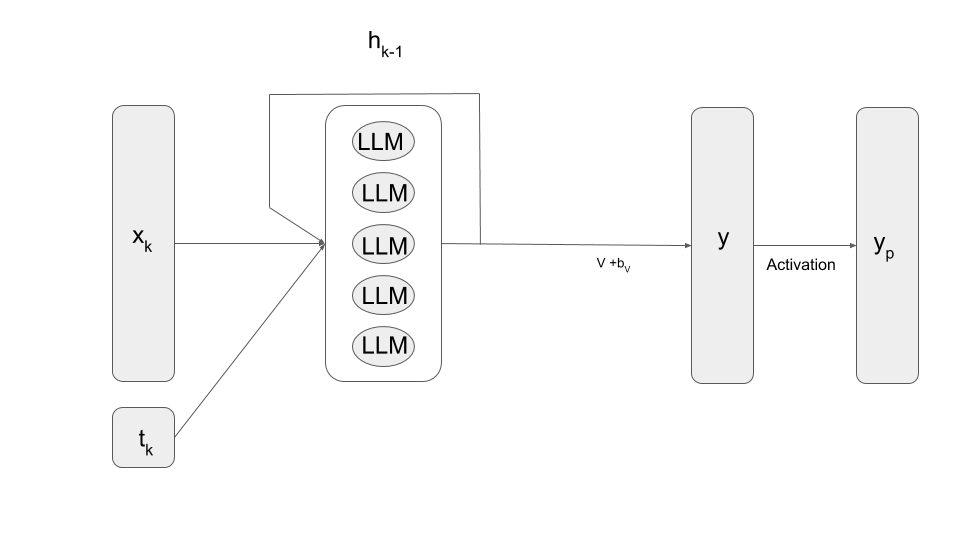
\includegraphics[width=1.0\textwidth]{figures/LLM_Network.png}}
    \caption{Lifetime Limited Memory Network}
    \label{fig:LLMNet}
    Overall structure of the LLM network
    
            
    \end{center}
\end{figure}
\begin{figure}

\begin{center}
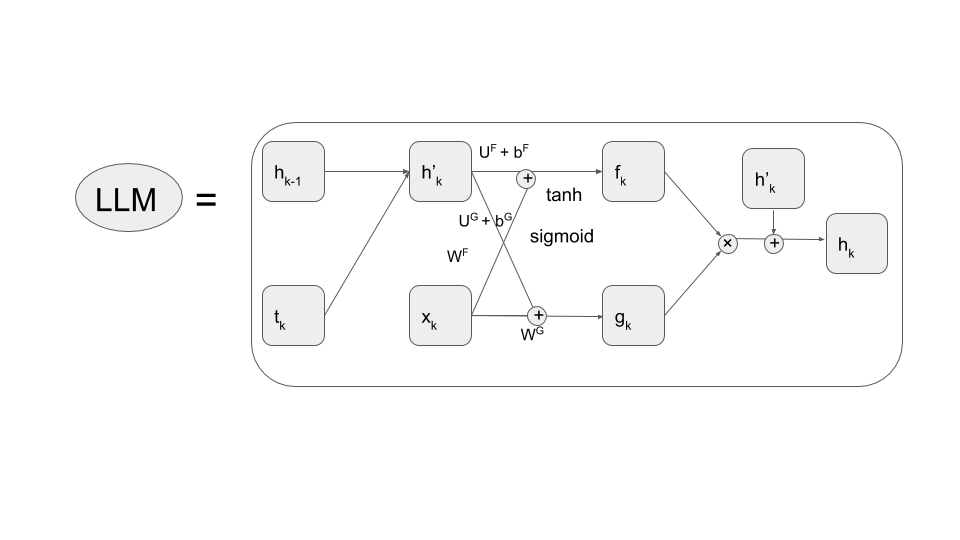
\includegraphics[width=1.0\textwidth]{figures/LLM_Cell.png}
    \caption{Lifetime Limited Memory Cell}
    \label{fig:LLMCell}
    Internal structure of the LLM hidden cell
    
    \end{center}
\end{figure}